% last updated in April 2002 by Antje Endemann
% Based on CVPR 07 and LNCS, with modifications by DAF, AZ and elle, 2008 and AA, 2010, and CC, 2011; TT, 2014; AAS, 2016

\documentclass[runningheads]{llncs}
\usepackage{graphicx}
\usepackage{amsmath,amssymb} % define this before the line numbering.
\usepackage{ruler}
\usepackage{times}
\usepackage{epsfig}
\usepackage{url}
\usepackage{subfigure}
\usepackage{lineno}
\usepackage{setspace}
\usepackage{upgreek}
\usepackage{authblk}
\usepackage{xpatch}
\usepackage{color}
\usepackage{morefloats}
\usepackage[width=122mm,left=12mm,paperwidth=146mm,height=193mm,top=12mm,paperheight=217mm]{geometry}

\begin{document}

\pagestyle{headings}
\mainmatter
\def\ECCV16SubNumber{***}  % Insert your submission number here

\title{Supplementary Material to ``Patch Group based Bayesian Learning for Blind Image Denoising"} % Replace with your title
\titlerunning{Supplementary Material} % Replace with your title

\authorrunning{Jun Xu, Dongwei Ren, Lei Zhang, David Zhang}
\author{Jun Xu$^{1}$, Dongwei Ren$^{1,2}$, Lei Zhang$^{1}$\footnote{This work is supported by the HK RGC GRF grant (PolyU5313/12E).}, David Zhang$^{1}$} % Replace with your names
\institute{$^{1}$Dept. of Computing, The Hong Kong Polytechnic University, Hong Kong, China\\
$^{2}$School of Computer Science and Technology, Harbin Institute of Technology, Harbin, China}


\maketitle

In this supplementary material, we provide:
\begin{enumerate}
\item More denoising results on the 20 natural images corrupted by Gaussian noise;
\item More denoising results on the 20 natural images corrupted by mixed Gaussian and Random Value Impulse Noise (RVIN);
\item More denoising results on real noisy images;
\item Visual comparison with the PGPD algorithm.
\end{enumerate}

\section{More Results on Gaussian Noise Removal}
In the main paper, we had given some examples of Gaussian noise removal on the 20 widely used images. We compared the proposed method with BM3D \cite{bm3d}, WNNM \cite{wnnm}, Two Phase \cite{cai2010fast}, WESNR \cite{wesnr}, Noise Clinic \cite{noiseclinic}. In Figures \ref{fig1}-\ref{fig8}, we give more visual comparisons of those competing methods \cite{bm3d,wnnm,cai2010fast,wesnr,noiseclinic}.
\begin{figure}
\centering
\subfigure{
\begin{minipage}[t]{0.244\textwidth}
\centering
\raisebox{-0.15cm}{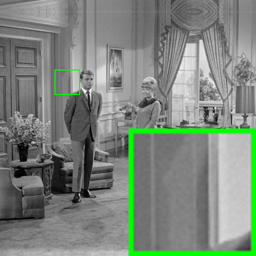
\includegraphics[width=1\textwidth]{Gaussian/resize_br_Original_couple.png}}
{\footnotesize (a) Ground Truth}
\end{minipage}
\begin{minipage}[t]{0.244\textwidth}
\centering
\raisebox{-0.15cm}{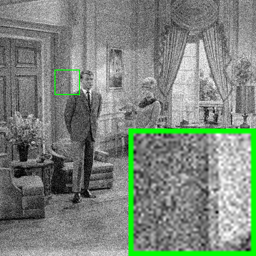
\includegraphics[width=1\textwidth]{Gaussian/resize_br_Noisy_Gau_30_couple.png}}
{\footnotesize (b) Noisy Image \\(18.73dB/0.3128)}
\end{minipage}
\begin{minipage}[t]{0.244\textwidth}
\centering
\raisebox{-0.15cm}{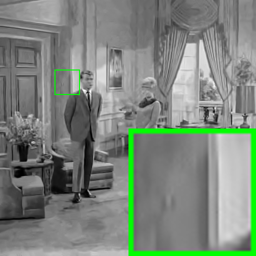
\includegraphics[width=1\textwidth]{Gaussian/resize_br_BM3D_Gau_30_couple.png}}
{\footnotesize (c) BM3D \\(28.86dB/0.7941)}
\end{minipage}
\begin{minipage}[t]{0.244\textwidth}
\centering
\raisebox{-0.15cm}{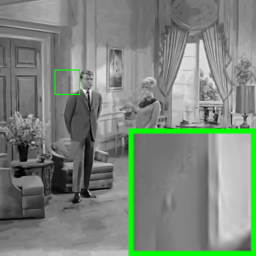
\includegraphics[width=1\textwidth]{Gaussian/resize_br_WNNM_Gau_30_couple.png}}
{\footnotesize (d) WNNM \\(28.98dB/0.7952)}
\end{minipage}
}
\subfigure{
\begin{minipage}[t]{0.244\textwidth}
\centering
\raisebox{-0.15cm}{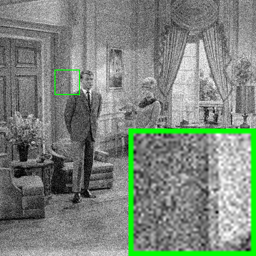
\includegraphics[width=1\textwidth]{Gaussian/resize_br_TwoPhase_Gau_30_couple.png}}
{\footnotesize (e) Two Phase \\(18.73dB/0.3128)}
\end{minipage}
\begin{minipage}[t]{0.244\textwidth}
\centering
\raisebox{-0.15cm}{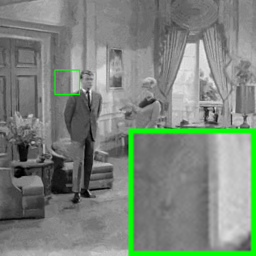
\includegraphics[width=1\textwidth]{Gaussian/resize_br_WESNR_Gau_30_couple.png}}
{\footnotesize (f) WESNR \\(27.23dB/0.7176)}
\end{minipage}
\begin{minipage}[t]{0.244\textwidth}
\centering
\raisebox{-0.15cm}{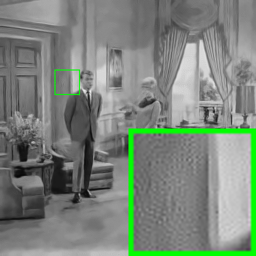
\includegraphics[width=1\textwidth]{Gaussian/resize_br_NC_Gau_30_couple.png}}
{\footnotesize (g) Noise Clinic \\(26.68dB/0.6339)}
\end{minipage}
\begin{minipage}[t]{0.244\textwidth}
\centering
\raisebox{-0.15cm}{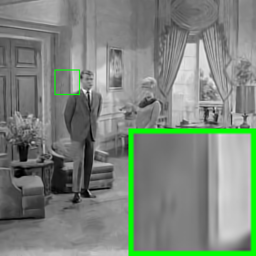
\includegraphics[width=1\textwidth]{Gaussian/resize_br_Ours_Gau_30_couple.png}}
{\footnotesize (h) Ours \\(28.27dB/0.7737)}
\end{minipage}
}
\caption{Denoised images of \textsl{Couple} and PSNR/SSIM results by different methods (the standard deviation of Gaussian noise is $\sigma=30$).}
\label{fig1}
\end{figure}

\begin{figure}
\centering
\subfigure{
\begin{minipage}[t]{0.244\textwidth}
\centering
\raisebox{-0.15cm}{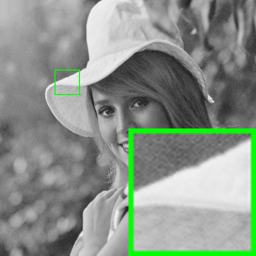
\includegraphics[width=1\textwidth]{Gaussian/resize_br_Original_elaine.png}}
{\footnotesize (a) Ground Truth}
\end{minipage}
\begin{minipage}[t]{0.244\textwidth}
\centering
\raisebox{-0.15cm}{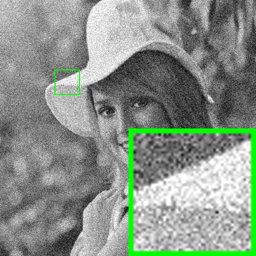
\includegraphics[width=1\textwidth]{Gaussian/resize_br_Noisy_Gau_30_elaine.png}}
{\footnotesize (b) Noisy Image \\(18.72dB/0.2138)}
\end{minipage}
\begin{minipage}[t]{0.244\textwidth}
\centering
\raisebox{-0.15cm}{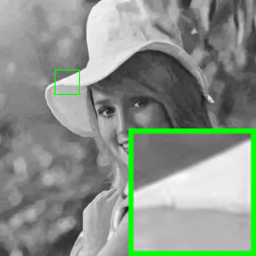
\includegraphics[width=1\textwidth]{Gaussian/resize_br_BM3D_Gau_30_elaine.png}}
{\footnotesize (c) BM3D \\(30.45dB/0.7263)}
\end{minipage}
\begin{minipage}[t]{0.244\textwidth}
\centering
\raisebox{-0.15cm}{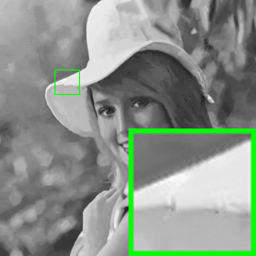
\includegraphics[width=1\textwidth]{Gaussian/resize_br_WNNM_Gau_30_elaine.png}}
{\footnotesize (d) WNNM \\(30.45dB/0.7270)}
\end{minipage}
}
\subfigure{
\begin{minipage}[t]{0.244\textwidth}
\centering
\raisebox{-0.15cm}{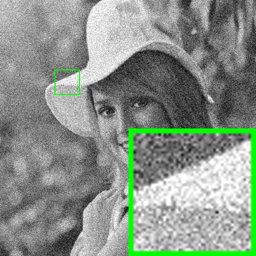
\includegraphics[width=1\textwidth]{Gaussian/resize_br_TwoPhase_Gau_30_elaine.png}}
{\footnotesize (e) Two Phase \\(18.72dB/0.2138)}
\end{minipage}
\begin{minipage}[t]{0.244\textwidth}
\centering
\raisebox{-0.15cm}{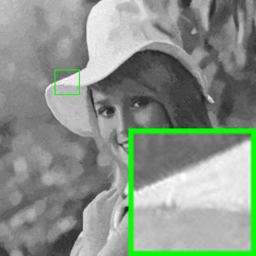
\includegraphics[width=1\textwidth]{Gaussian/resize_br_WESNR_Gau_30_elaine.png}}
{\footnotesize (f) WESNR \\(29.42dB/0.6825)}
\end{minipage}
\begin{minipage}[t]{0.244\textwidth}
\centering
\raisebox{-0.15cm}{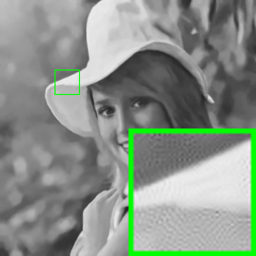
\includegraphics[width=1\textwidth]{Gaussian/resize_br_NC_Gau_30_elaine.png}}
{\footnotesize (g) Noise Clinic \\(28.34dB/0.6103)}
\end{minipage}
\begin{minipage}[t]{0.244\textwidth}
\centering
\raisebox{-0.15cm}{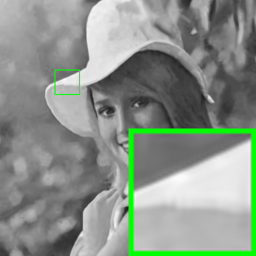
\includegraphics[width=1\textwidth]{Gaussian/resize_br_Ours_Gau_30_elaine.png}}
{\footnotesize (h) Ours \\(30.41dB/0.7212)}
\end{minipage}
}
\caption{Denoised images of \textsl{Elaine} and PSNR/SSIM results by different methods (the standard deviation of Gaussian noise is $\sigma=30$).}
\label{fig2}
\end{figure}

\begin{figure}
\centering
\subfigure{
\begin{minipage}[t]{0.244\textwidth}
\centering
\raisebox{-0.15cm}{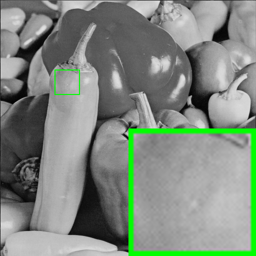
\includegraphics[width=1\textwidth]{Gaussian/resize_br_Original_peppers.png}}
{\footnotesize (a) Ground Truth}
\end{minipage}
\begin{minipage}[t]{0.244\textwidth}
\centering
\raisebox{-0.15cm}{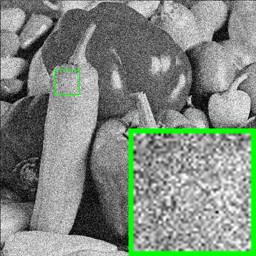
\includegraphics[width=1\textwidth]{Gaussian/resize_br_Noisy_Gau_40_peppers.png}}
{\footnotesize (b) Noisy Image \\(16.45dB/0.1548)}
\end{minipage}
\begin{minipage}[t]{0.244\textwidth}
\centering
\raisebox{-0.15cm}{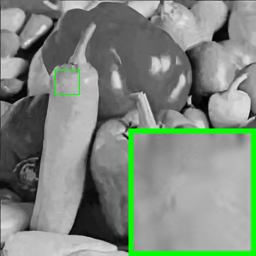
\includegraphics[width=1\textwidth]{Gaussian/resize_br_BM3D_Gau_40_peppers.png}}
{\footnotesize (c) BM3D \\(29.97dB/0.7950)}
\end{minipage}
\begin{minipage}[t]{0.244\textwidth}
\centering
\raisebox{-0.15cm}{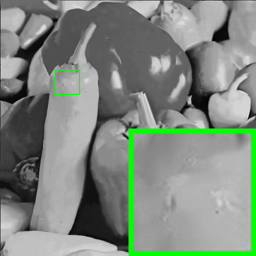
\includegraphics[width=1\textwidth]{Gaussian/resize_br_WNNM_Gau_40_peppers.png}}
{\footnotesize (d) WNNM \\(30.17dB/0.8003)}
\end{minipage}
}
\subfigure{
\begin{minipage}[t]{0.244\textwidth}
\centering
\raisebox{-0.15cm}{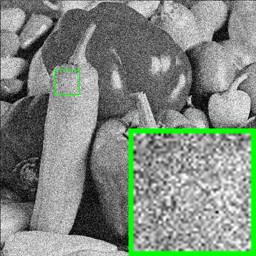
\includegraphics[width=1\textwidth]{Gaussian/resize_br_TwoPhase_Gau_40_peppers.png}}
{\footnotesize (e) Two Phase \\(16.45dB/0.1548)}
\end{minipage}
\begin{minipage}[t]{0.244\textwidth}
\centering
\raisebox{-0.15cm}{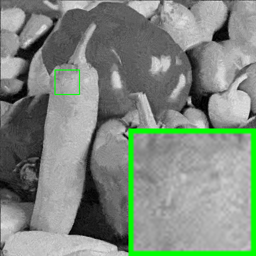
\includegraphics[width=1\textwidth]{Gaussian/resize_br_WESNR_Gau_40_peppers.png}}
{\footnotesize (f) WESNR \\(26.98dB/0.5969)}
\end{minipage}
\begin{minipage}[t]{0.244\textwidth}
\centering
\raisebox{-0.15cm}{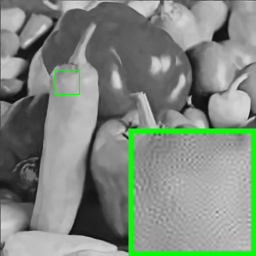
\includegraphics[width=1\textwidth]{Gaussian/resize_br_NC_Gau_40_peppers.png}}
{\footnotesize (g) Noise Clinic \\(26.41dB/0.5443)}
\end{minipage}
\begin{minipage}[t]{0.244\textwidth}
\centering
\raisebox{-0.15cm}{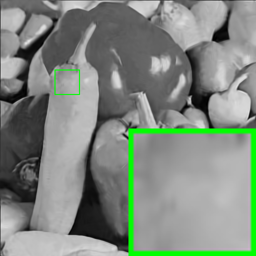
\includegraphics[width=1\textwidth]{Gaussian/resize_br_Ours_Gau_40_peppers.png}}
{\footnotesize (h) Ours \\(30.01dB/0.8008)}
\end{minipage}
}
\caption{Denoised images of \textsl{Peppers} and PSNR/SSIM results by different methods (the standard deviation of Gaussian noise is $\sigma=40$).}
\label{fig3}
\end{figure}

\begin{figure}
\centering
\subfigure{
\begin{minipage}[t]{0.244\textwidth}
\centering
\raisebox{-0.15cm}{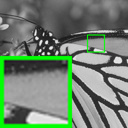
\includegraphics[width=1\textwidth]{Gaussian/resize_br_Original_monarch.png}}
{\footnotesize (a) Ground Truth}
\end{minipage}
\begin{minipage}[t]{0.244\textwidth}
\centering
\raisebox{-0.15cm}{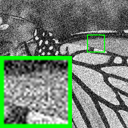
\includegraphics[width=1\textwidth]{Gaussian/resize_br_Noisy_Gau_40_monarch.png}}
{\footnotesize (b) Noisy Image \\(16.41dB/0.3131)}
\end{minipage}
\begin{minipage}[t]{0.244\textwidth}
\centering
\raisebox{-0.15cm}{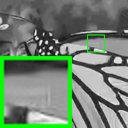
\includegraphics[width=1\textwidth]{Gaussian/resize_br_BM3D_Gau_40_monarch.png}}
{\footnotesize (c) BM3D \\(26.68dB/0.8413)}
\end{minipage}
\begin{minipage}[t]{0.244\textwidth}
\centering
\raisebox{-0.15cm}{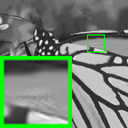
\includegraphics[width=1\textwidth]{Gaussian/resize_br_WNNM_Gau_40_monarch.png}}
{\footnotesize (d) WNNM \\(27.44dB/0.8557)}
\end{minipage}
}
\subfigure{
\begin{minipage}[t]{0.244\textwidth}
\centering
\raisebox{-0.15cm}{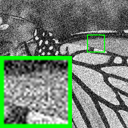
\includegraphics[width=1\textwidth]{Gaussian/resize_br_TwoPhase_Gau_40_monarch.png}}
{\footnotesize (e) Two Phase \\(16.41dB/0.3131)}
\end{minipage}
\begin{minipage}[t]{0.244\textwidth}
\centering
\raisebox{-0.15cm}{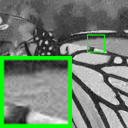
\includegraphics[width=1\textwidth]{Gaussian/resize_br_WESNR_Gau_40_monarch.png}}
{\footnotesize (f) WESNR \\(23.30dB/0.6754)}
\end{minipage}
\begin{minipage}[t]{0.244\textwidth}
\centering
\raisebox{-0.15cm}{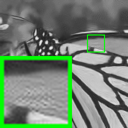
\includegraphics[width=1\textwidth]{Gaussian/resize_br_NC_Gau_40_monarch.png}}
{\footnotesize (g) Noise Clinic \\(25.22dB/0.6812)}
\end{minipage}
\begin{minipage}[t]{0.244\textwidth}
\centering
\raisebox{-0.15cm}{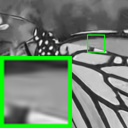
\includegraphics[width=1\textwidth]{Gaussian/resize_br_Ours_Gau_40_monarch.png}}
{\footnotesize (h) Ours \\(26.57dB/0.8487)}
\end{minipage}
}
\caption{Denoised images of \textsl{Monarch} and PSNR/SSIM results by different methods (the standard deviation of Gaussian noise is $\sigma=40$).}
\label{fig4}
\end{figure}

\begin{figure}
\centering
\subfigure{
\begin{minipage}[t]{0.244\textwidth}
\centering
\raisebox{-0.15cm}{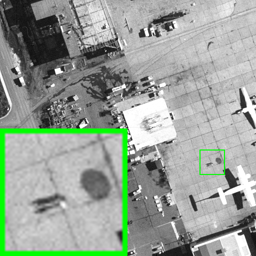
\includegraphics[width=1\textwidth]{Gaussian/resize_br_Original_airfield.png}}
{\footnotesize (a) Ground Truth}
\end{minipage}
\begin{minipage}[t]{0.244\textwidth}
\centering
\raisebox{-0.15cm}{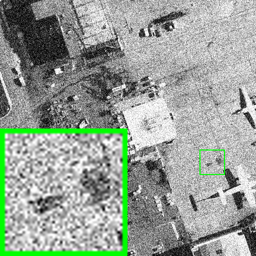
\includegraphics[width=1\textwidth]{Gaussian/resize_br_Noisy_Gau_50_airfield.png}}
{\footnotesize (b) Noisy Image \\(14.88dB/0.2394)}
\end{minipage}
\begin{minipage}[t]{0.244\textwidth}
\centering
\raisebox{-0.15cm}{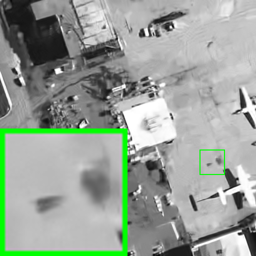
\includegraphics[width=1\textwidth]{Gaussian/resize_br_BM3D_Gau_50_airfield.png}}
{\footnotesize (c) BM3D \\(24.19dB/0.5977)}
\end{minipage}
\begin{minipage}[t]{0.244\textwidth}
\centering
\raisebox{-0.15cm}{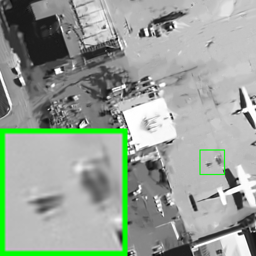
\includegraphics[width=1\textwidth]{Gaussian/resize_br_WNNM_Gau_50_airfield.png}}
{\footnotesize (d) WNNM \\(24.51dB/0.6095)}
\end{minipage}
}
\subfigure{
\begin{minipage}[t]{0.244\textwidth}
\centering
\raisebox{-0.15cm}{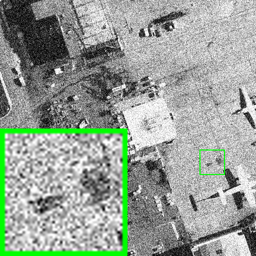
\includegraphics[width=1\textwidth]{Gaussian/resize_br_TwoPhase_Gau_50_airfield.png}}
{\footnotesize (e) Two Phase \\(14.88dB/0.2394)}
\end{minipage}
\begin{minipage}[t]{0.244\textwidth}
\centering
\raisebox{-0.15cm}{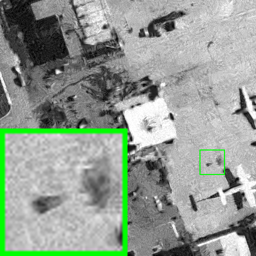
\includegraphics[width=1\textwidth]{Gaussian/resize_br_WESNR_Gau_50_airfield.png}}
{\footnotesize (f) WESNR \\(17.89dB/0.4126)}
\end{minipage}
\begin{minipage}[t]{0.244\textwidth}
\centering
\raisebox{-0.15cm}{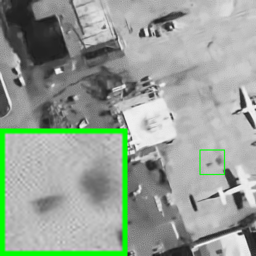
\includegraphics[width=1\textwidth]{Gaussian/resize_br_NC_Gau_50_airfield.png}}
{\footnotesize (g) Noise Clinic \\(22.31dB/0.4867)}
\end{minipage}
\begin{minipage}[t]{0.244\textwidth}
\centering
\raisebox{-0.15cm}{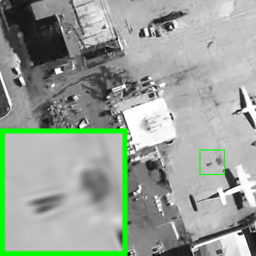
\includegraphics[width=1\textwidth]{Gaussian/resize_br_Ours_Gau_50_airfield.png}}
{\footnotesize (h) Ours \\(24.12dB/0.5910)}
\end{minipage}
}
\caption{Denoised images of \textsl{Airfield} and PSNR/SSIM results by different methods (the standard deviation of Gaussian noise is $\sigma=50$).}
\label{fig5}
\end{figure}


\begin{figure}
\centering
\subfigure{
\begin{minipage}[t]{0.244\textwidth}
\centering
\raisebox{-0.15cm}{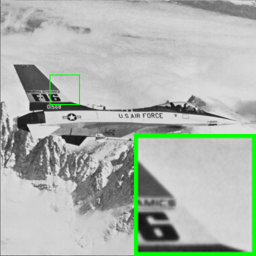
\includegraphics[width=1\textwidth]{Gaussian/resize_br_Original_airplane.png}}
{\footnotesize (a) Ground Truth}
\end{minipage}
\begin{minipage}[t]{0.244\textwidth}
\centering
\raisebox{-0.15cm}{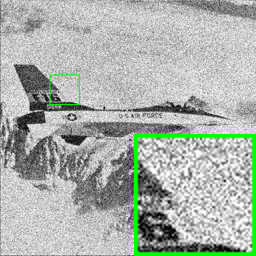
\includegraphics[width=1\textwidth]{Gaussian/resize_br_Noisy_Gau_50_airplane.png}}
{\footnotesize (b) Noisy Image \\(15.08dB/0.1370)}
\end{minipage}
\begin{minipage}[t]{0.244\textwidth}
\centering
\raisebox{-0.15cm}{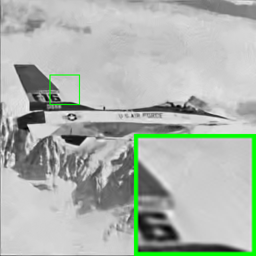
\includegraphics[width=1\textwidth]{Gaussian/resize_br_BM3D_Gau_50_airplane.png}}
{\footnotesize (c) BM3D \\(28.24dB/0.8253)}
\end{minipage}
\begin{minipage}[t]{0.244\textwidth}
\centering
\raisebox{-0.15cm}{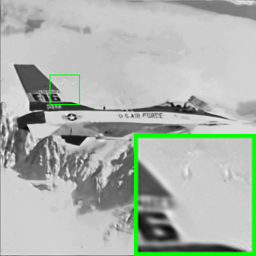
\includegraphics[width=1\textwidth]{Gaussian/resize_br_WNNM_Gau_50_airplane.png}}
{\footnotesize (d) WNNM \\(28.55dB/0.8279)}
\end{minipage}
}
\subfigure{
\begin{minipage}[t]{0.244\textwidth}
\centering
\raisebox{-0.15cm}{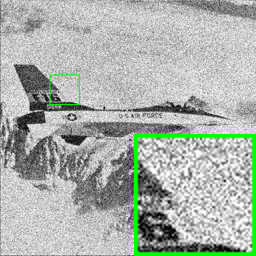
\includegraphics[width=1\textwidth]{Gaussian/resize_br_TwoPhase_Gau_50_airplane.png}}
{\footnotesize (e) Two Phase \\(15.08dB/0.1370)}
\end{minipage}
\begin{minipage}[t]{0.244\textwidth}
\centering
\raisebox{-0.15cm}{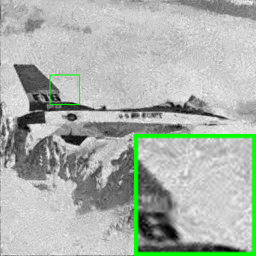
\includegraphics[width=1\textwidth]{Gaussian/resize_br_WESNR_Gau_50_airplane.png}}
{\footnotesize (f) WESNR \\(23.14dB/0.4278)}
\end{minipage}
\begin{minipage}[t]{0.244\textwidth}
\centering
\raisebox{-0.15cm}{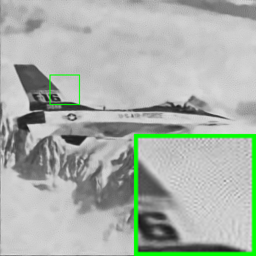
\includegraphics[width=1\textwidth]{Gaussian/resize_br_NC_Gau_50_airplane.png}}
{\footnotesize (g) Noise Clinic \\(25.02dB/0.5122)}
\end{minipage}
\begin{minipage}[t]{0.244\textwidth}
\centering
\raisebox{-0.15cm}{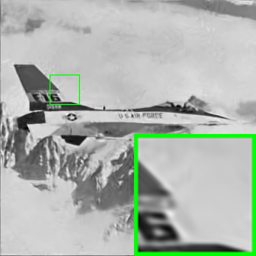
\includegraphics[width=1\textwidth]{Gaussian/resize_br_Ours_Gau_50_airplane.png}}
{\footnotesize (h) Ours \\(28.18dB/0.8295)}
\end{minipage}
}
\caption{Denoised images of \textsl{Airplane} and PSNR/SSIM results by different methods (the standard deviation of Gaussian noise is $\sigma=50$).}
\label{fig6}
\end{figure}

\begin{figure}
\centering
\subfigure{
\begin{minipage}[t]{0.244\textwidth}
\centering
\raisebox{-0.15cm}{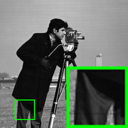
\includegraphics[width=1\textwidth]{Gaussian/resize_br_Original_cameraman.png}}
{\footnotesize (a) Ground Truth}
\end{minipage}
\begin{minipage}[t]{0.244\textwidth}
\centering
\raisebox{-0.15cm}{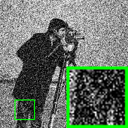
\includegraphics[width=1\textwidth]{Gaussian/resize_br_Noisy_Gau_75_cameraman.png}}
{\footnotesize (b) Noisy Image \\(10.60dB/0.1125)}
\end{minipage}
\begin{minipage}[t]{0.244\textwidth}
\centering
\raisebox{-0.15cm}{\includegraphics[width=1\textwidth]{Gaussian/resize_br_BM3D_Gau_75_cameraman.png}}
{\footnotesize (c) BM3D \\(24.34dB/0.7319)}
\end{minipage}
\begin{minipage}[t]{0.244\textwidth}
\centering
\raisebox{-0.15cm}{\includegraphics[width=1\textwidth]{Gaussian/resize_br_WNNM_Gau_75_cameraman.png}}
{\footnotesize (d) WNNM \\(24.53dB/0.7306)}
\end{minipage}
}
\subfigure{
\begin{minipage}[t]{0.244\textwidth}
\centering
\raisebox{-0.15cm}{\includegraphics[width=1\textwidth]{Gaussian/resize_br_TwoPhase_Gau_75_cameraman.png}}
{\footnotesize (e) Two Phase \\(11.97dB/0.1287)}
\end{minipage}
\begin{minipage}[t]{0.244\textwidth}
\centering
\raisebox{-0.15cm}{\includegraphics[width=1\textwidth]{Gaussian/resize_br_WESNR_Gau_75_cameraman.png}}
{\footnotesize (f) WESNR \\(9.56dB/0.1913)}
\end{minipage}
\begin{minipage}[t]{0.244\textwidth}
\centering
\raisebox{-0.15cm}{\includegraphics[width=1\textwidth]{Gaussian/resize_br_NC_Gau_75_cameraman.png}}
{\footnotesize (g) Noise Clinic \\(16.42dB/0.2429)}
\end{minipage}
\begin{minipage}[t]{0.244\textwidth}
\centering
\raisebox{-0.15cm}{\includegraphics[width=1\textwidth]{Gaussian/resize_br_Ours_Gau_75_cameraman.png}}
{\footnotesize (h) Ours \\(24.33dB/0.7321)}
\end{minipage}
}
\caption{Denoised images of \textsl{Cameraman} and PSNR/SSIM results by different methods (the standard deviation of Gaussian noise is $\sigma=75$).}
\label{fig7}
\end{figure}

\begin{figure}
\centering
\subfigure{
\begin{minipage}[t]{0.244\textwidth}
\centering
\raisebox{-0.15cm}{\includegraphics[width=1\textwidth]{Gaussian/resize_br_Original_leaves.png}}
{\footnotesize (a) Ground Truth}
\end{minipage}
\begin{minipage}[t]{0.244\textwidth}
\centering
\raisebox{-0.15cm}{\includegraphics[width=1\textwidth]{Gaussian/resize_br_Noisy_Gau_75_leaves.png}}
{\footnotesize (b) Noisy Image \\(10.60dB/0.2658)}
\end{minipage}
\begin{minipage}[t]{0.244\textwidth}
\centering
\raisebox{-0.15cm}{\includegraphics[width=1\textwidth]{Gaussian/resize_br_BM3D_Gau_75_leaves.png}}
{\footnotesize (c) BM3D \\(22.50dB/0.8067)}
\end{minipage}
\begin{minipage}[t]{0.244\textwidth}
\centering
\raisebox{-0.15cm}{\includegraphics[width=1\textwidth]{Gaussian/resize_br_WNNM_Gau_75_leaves.png}}
{\footnotesize (d) WNNM \\(23.00dB/0.8300)}
\end{minipage}
}
\subfigure{
\begin{minipage}[t]{0.244\textwidth}
\centering
\raisebox{-0.15cm}{\includegraphics[width=1\textwidth]{Gaussian/resize_br_TwoPhase_Gau_75_leaves.png}}
{\footnotesize (e) Two Phase \\(12.55dB/0.3074)}
\end{minipage}
\begin{minipage}[t]{0.244\textwidth}
\centering
\raisebox{-0.15cm}{\includegraphics[width=1\textwidth]{Gaussian/br_WESNR_Gau_75_leaves.png}}
{\footnotesize (f) WESNR \\(4.25dB/0.0.0755)}
\end{minipage}
\begin{minipage}[t]{0.244\textwidth}
\centering
\raisebox{-0.15cm}{\includegraphics[width=1\textwidth]{Gaussian/resize_br_NC_Gau_75_leaves.png}}
{\footnotesize (g) Noise Clinic \\(17.83dB/0.5498)}
\end{minipage}
\begin{minipage}[t]{0.244\textwidth}
\centering
\raisebox{-0.15cm}{\includegraphics[width=1\textwidth]{Gaussian/resize_br_Ours_Gau_75_leaves.png}}
{\footnotesize (h) Ours \\(22.35dB/0.7931)}
\end{minipage}
}
\caption{Denoised images of \textsl{Leaves} and PSNR/SSIM results by different methods (the standard deviation of Gaussian noise is $\sigma=75$).}
\label{fig8}
\end{figure}

\section{More Results on Mixed Gaussian and Random Vaule Impulse Noise Removal}
In the main paper, we had given some examples of mixed Gaussian and random value impulse noise removal on the 20 widely used images. In this section, we give more visual comparisons of the proposed method with BM3D \cite{bm3d}, WNNM \cite{wnnm}, Two Phase \cite{cai2010fast}, WESNR \cite{wesnr}, Noise Clinic \cite{noiseclinic} in Figures \ref{fig9}-\ref{fig16}.
\begin{figure}
\centering
\subfigure{
\begin{minipage}[t]{0.244\textwidth}
\centering
\raisebox{-0.15cm}{\includegraphics[width=1\textwidth]{GRVIN/resize_br_Original_airfield.png}}
{\footnotesize (a) Ground Truth}
\end{minipage}
\begin{minipage}[t]{0.244\textwidth}
\centering
\raisebox{-0.15cm}{\includegraphics[width=1\textwidth]{GRVIN/resize_br_Noisy_GauRVIN_10_015_airfield.png}}
{\footnotesize (b) Noisy Image \\(16.47dB/0.3308)}
\end{minipage}
\begin{minipage}[t]{0.244\textwidth}
\centering
\raisebox{-0.15cm}{\includegraphics[width=1\textwidth]{GRVIN/resize_br_BM3D_GauRVIN_10_015_airfield.png}}
{\footnotesize (c) BM3D \\(22.82dB/0.5653)}
\end{minipage}
\begin{minipage}[t]{0.244\textwidth}
\centering
\raisebox{-0.15cm}{\includegraphics[width=1\textwidth]{GRVIN/resize_br_WNNM_GauRVIN_10_015_airfield.png}}
{\footnotesize (d) WNNM \\(21.59dB/0.4967)}
\end{minipage}
}
\subfigure{
\begin{minipage}[t]{0.244\textwidth}
\centering
\raisebox{-0.15cm}{\includegraphics[width=1\textwidth]{GRVIN/resize_br_TwoPhase_GauRVIN_10_015_airfield.png}}
{\footnotesize (e) Two Phase \\(25.41dB/0.7173)}
\end{minipage}
\begin{minipage}[t]{0.244\textwidth}
\centering
\raisebox{-0.15cm}{\includegraphics[width=1\textwidth]{GRVIN/resize_br_WESNR_GauRVIN_10_015_airfield.png}}
{\footnotesize (f) WESNR \\(23.85dB/0.6919)}
\end{minipage}
\begin{minipage}[t]{0.244\textwidth}
\centering
\raisebox{-0.15cm}{\includegraphics[width=1\textwidth]{GRVIN/resize_br_NC_GauRVIN_10_015_airfield.png}}
{\footnotesize (g) Noise Clinic \\(18.18dB/0.3604)}
\end{minipage}
\begin{minipage}[t]{0.244\textwidth}
\centering
\raisebox{-0.15cm}{\includegraphics[width=1\textwidth]{GRVIN/resize_br_Ours_GauRVIN_10_015_airfield.png}}
{\footnotesize (h) Ours \\(24.49dB/0.6177)}
\end{minipage}
}
\caption{Denoised images of \textsl{Airfield} by different methods (the mixed Gaussian and RVIN noise is with $\sigma = 10$ and ratio $0.15$).}
\label{fig9}
\end{figure}

\begin{figure}
\centering
\subfigure{
\begin{minipage}[t]{0.244\textwidth}
\centering
\raisebox{-0.15cm}{\includegraphics[width=1\textwidth]{GRVIN/resize_br_Original_baboon.png}}
{\footnotesize (a) Ground Truth}
\end{minipage}
\begin{minipage}[t]{0.244\textwidth}
\centering
\raisebox{-0.15cm}{\includegraphics[width=1\textwidth]{GRVIN/resize_br_Noisy_GauRVIN_10_015_baboon.png}}
{\footnotesize (b) Noisy Image \\(17.49dB/0.4275)}
\end{minipage}
\begin{minipage}[t]{0.244\textwidth}
\centering
\raisebox{-0.15cm}{\includegraphics[width=1\textwidth]{GRVIN/resize_br_BM3D_GauRVIN_10_015_baboon.png}}
{\footnotesize (c) BM3D \\(22.83dB/0.5952)}
\end{minipage}
\begin{minipage}[t]{0.244\textwidth}
\centering
\raisebox{-0.15cm}{\includegraphics[width=1\textwidth]{GRVIN/resize_br_WNNM_GauRVIN_10_015_baboon.png}}
{\footnotesize (d) WNNM \\(22.27dB/0.5548)}
\end{minipage}
}
\subfigure{
\begin{minipage}[t]{0.244\textwidth}
\centering
\raisebox{-0.15cm}{\includegraphics[width=1\textwidth]{GRVIN/resize_br_TwoPhase_GauRVIN_10_015_baboon.png}}
{\footnotesize (e) Two Phase \\(22.94dB/0.6717)}
\end{minipage}
\begin{minipage}[t]{0.244\textwidth}
\centering
\raisebox{-0.15cm}{\includegraphics[width=1\textwidth]{GRVIN/resize_br_WESNR_GauRVIN_10_015_baboon.png}}
{\footnotesize (f) WESNR \\(24.49dB/0.7261)}
\end{minipage}
\begin{minipage}[t]{0.244\textwidth}
\centering
\raisebox{-0.15cm}{\includegraphics[width=1\textwidth]{GRVIN/resize_br_NC_GauRVIN_10_015_baboon.png}}
{\footnotesize (g) Noise Clinic \\(19.52dB/0.4463)}
\end{minipage}
\begin{minipage}[t]{0.244\textwidth}
\centering
\raisebox{-0.15cm}{\includegraphics[width=1\textwidth]{GRVIN/resize_br_Ours_GauRVIN_10_015_baboon.png}}
{\footnotesize (h) Ours \\(23.01dB/0.5963)}
\end{minipage}
}
\caption{Denoised images of \textsl{Baboon} by different methods (the mixed Gaussian and RVIN noise is with $\sigma = 10$ and ratio $0.15$).}
\label{fig10}
\end{figure}

\begin{figure}
\centering
\subfigure{
\begin{minipage}[t]{0.244\textwidth}
\centering
\raisebox{-0.15cm}{\includegraphics[width=1\textwidth]{GRVIN/resize_br_Original_airplane.png}}
{\footnotesize (a) Ground Truth}
\end{minipage}
\begin{minipage}[t]{0.244\textwidth}
\centering
\raisebox{-0.15cm}{\includegraphics[width=1\textwidth]{GRVIN/resize_br_Noisy_GauRVIN_10_030_airplane.png}}
{\footnotesize (b) Noisy Image \\(13.22dB/0.1161)}
\end{minipage}
\begin{minipage}[t]{0.244\textwidth}
\centering
\raisebox{-0.15cm}{\includegraphics[width=1\textwidth]{GRVIN/resize_br_BM3D_GauRVIN_10_030_airplane.png}}
{\footnotesize (c) BM3D \\(21.42dB/0.7517)}
\end{minipage}
\begin{minipage}[t]{0.244\textwidth}
\centering
\raisebox{-0.15cm}{\includegraphics[width=1\textwidth]{GRVIN/resize_br_WNNM_GauRVIN_10_030_airplane.png}}
{\footnotesize (d) WNNM \\(20.99dB/0.6423)}
\end{minipage}
}
\subfigure{
\begin{minipage}[t]{0.244\textwidth}
\centering
\raisebox{-0.15cm}{\includegraphics[width=1\textwidth]{GRVIN/resize_br_TwoPhase_GauRVIN_10_030_airplane.png}}
{\footnotesize (e) Two Phase \\(27.09dB/0.6577)}
\end{minipage}
\begin{minipage}[t]{0.244\textwidth}
\centering
\raisebox{-0.15cm}{\includegraphics[width=1\textwidth]{GRVIN/resize_br_WESNR_GauRVIN_10_030_airplane.png}}
{\footnotesize (f) WESNR \\(20.54dB/0.3907)}
\end{minipage}
\begin{minipage}[t]{0.244\textwidth}
\centering
\raisebox{-0.15cm}{\includegraphics[width=1\textwidth]{GRVIN/resize_br_NC_GauRVIN_10_030_airplane.png}}
{\footnotesize (g) Noise Clinic \\(15.54dB/0.1467)}
\end{minipage}
\begin{minipage}[t]{0.244\textwidth}
\centering
\raisebox{-0.15cm}{\includegraphics[width=1\textwidth]{GRVIN/resize_br_Ours_GauRVIN_10_030_airplane.png}}
{\footnotesize (h) Ours \\(21.94dB/0.7680)}
\end{minipage}
}
\caption{Denoised images of \textsl{Airplane} by different methods (the mixed Gaussian and RVIN noise is with $\sigma = 10$ and ratio $0.3$).}
\label{fig11}
\end{figure}

\begin{figure}
\centering
\subfigure{
\begin{minipage}[t]{0.244\textwidth}
\centering
\raisebox{-0.15cm}{\includegraphics[width=1\textwidth]{GRVIN/resize_br_Original_peppers.png}}
{\footnotesize (a) Ground Truth}
\end{minipage}
\begin{minipage}[t]{0.244\textwidth}
\centering
\raisebox{-0.15cm}{\includegraphics[width=1\textwidth]{GRVIN/resize_br_Noisy_GauRVIN_10_030_peppers.png}}
{\footnotesize (b) Noisy Image \\(14.03dB/0.1054)}
\end{minipage}
\begin{minipage}[t]{0.244\textwidth}
\centering
\raisebox{-0.15cm}{\includegraphics[width=1\textwidth]{GRVIN/resize_br_BM3D_GauRVIN_10_030_peppers.png}}
{\footnotesize (c) BM3D \\(22.88dB/0.7084)}
\end{minipage}
\begin{minipage}[t]{0.244\textwidth}
\centering
\raisebox{-0.15cm}{\includegraphics[width=1\textwidth]{GRVIN/resize_br_WNNM_GauRVIN_10_030_peppers.png}}
{\footnotesize (d) WNNM \\(22.32dB/0.6664)}
\end{minipage}
}
\subfigure{
\begin{minipage}[t]{0.244\textwidth}
\centering
\raisebox{-0.15cm}{\includegraphics[width=1\textwidth]{GRVIN/resize_br_TwoPhase_GauRVIN_10_030_peppers.png}}
{\footnotesize (e) Two Phase \\(27.47dB/0.6562)}
\end{minipage}
\begin{minipage}[t]{0.244\textwidth}
\centering
\raisebox{-0.15cm}{\includegraphics[width=1\textwidth]{GRVIN/resize_br_WESNR_GauRVIN_10_030_peppers.png}}
{\footnotesize (f) WESNR \\(22.90dB/0.4645)}
\end{minipage}
\begin{minipage}[t]{0.244\textwidth}
\centering
\raisebox{-0.15cm}{\includegraphics[width=1\textwidth]{GRVIN/resize_br_NC_GauRVIN_10_030_peppers.png}}
{\footnotesize (g) Noise Clinic \\(16.67dB/0.1558)}
\end{minipage}
\begin{minipage}[t]{0.244\textwidth}
\centering
\raisebox{-0.15cm}{\includegraphics[width=1\textwidth]{GRVIN/resize_br_Ours_GauRVIN_10_030_peppers.png}}
{\footnotesize (h) Ours \\(23.49dB/0.7226)}
\end{minipage}
}
\caption{Denoised images of \textsl{Peppers} by different methods (the mixed Gaussian and RVIN noise is with $\sigma = 10$ and ratio $0.3$).}
\label{fig12}
\end{figure}

\begin{figure}
\centering
\subfigure{
\begin{minipage}[t]{0.244\textwidth}
\centering
\raisebox{-0.15cm}{\includegraphics[width=1\textwidth]{GRVIN/resize_br_Original_hill.png}}
{\footnotesize (a) Ground Truth}
\end{minipage}
\begin{minipage}[t]{0.244\textwidth}
\centering
\raisebox{-0.15cm}{\includegraphics[width=1\textwidth]{GRVIN/resize_br_Noisy_GauRVIN_20_015_hill.png}}
{\footnotesize (b) Noisy Image \\(16.22dB/0.1980)}
\end{minipage}
\begin{minipage}[t]{0.244\textwidth}
\centering
\raisebox{-0.15cm}{\includegraphics[width=1\textwidth]{GRVIN/resize_br_BM3D_GauRVIN_20_015_hill.png}}
{\footnotesize (c) BM3D \\(25.83dB/0.6429)}
\end{minipage}
\begin{minipage}[t]{0.244\textwidth}
\centering
\raisebox{-0.15cm}{\includegraphics[width=1\textwidth]{GRVIN/resize_br_WNNM_GauRVIN_20_015_hill.png}}
{\footnotesize (d) WNNM \\(23.65dB/0.5505)}
\end{minipage}
}
\subfigure{
\begin{minipage}[t]{0.244\textwidth}
\centering
\raisebox{-0.15cm}{\includegraphics[width=1\textwidth]{GRVIN/resize_br_TwoPhase_GauRVIN_20_015_hill.png}}
{\footnotesize (e) Two Phase \\(25.11dB/0.5275)}
\end{minipage}
\begin{minipage}[t]{0.244\textwidth}
\centering
\raisebox{-0.15cm}{\includegraphics[width=1\textwidth]{GRVIN/resize_br_WESNR_GauRVIN_20_015_hill.png}}
{\footnotesize (f) WESNR \\(28.08dB/0.7095)}
\end{minipage}
\begin{minipage}[t]{0.244\textwidth}
\centering
\raisebox{-0.15cm}{\includegraphics[width=1\textwidth]{GRVIN/resize_br_NC_GauRVIN_20_015_hill.png}}
{\footnotesize (g) Noise Clinic \\(20.45dB/0.3170)}
\end{minipage}
\begin{minipage}[t]{0.244\textwidth}
\centering
\raisebox{-0.15cm}{\includegraphics[width=1\textwidth]{GRVIN/resize_br_Ours_GauRVIN_20_015_hill.png}}
{\footnotesize (h) Ours \\(26.77dB/0.6706)}
\end{minipage}
}
\caption{Denoised images of \textsl{Hill} by different methods (the mixed Gaussian and RVIN noise is with $\sigma = 20$ and ratio $0.15$).}
\label{fig13}
\end{figure}

\begin{figure}
\centering
\subfigure{
\begin{minipage}[t]{0.244\textwidth}
\centering
\raisebox{-0.15cm}{\includegraphics[width=1\textwidth]{GRVIN/br_Original_house.png}}
{\footnotesize (a) Ground Truth}
\end{minipage}
\begin{minipage}[t]{0.244\textwidth}
\centering
\raisebox{-0.15cm}{\includegraphics[width=1\textwidth]{GRVIN/br_Noisy_GauRVIN_20_015_house.png}}
{\footnotesize (b) Noisy Image \\(16.36dB/0.1783)}
\end{minipage}
\begin{minipage}[t]{0.244\textwidth}
\centering
\raisebox{-0.15cm}{\includegraphics[width=1\textwidth]{GRVIN/br_BM3D_GauRVIN_20_015_house.png}}
{\footnotesize (c) BM3D \\(27.87dB/0.7856)}
\end{minipage}
\begin{minipage}[t]{0.244\textwidth}
\centering
\raisebox{-0.15cm}{\includegraphics[width=1\textwidth]{GRVIN/br_WNNM_GauRVIN_20_015_house.png}}
{\footnotesize (d) WNNM \\(25.13dB/0.6476)}
\end{minipage}
}
\subfigure{
\begin{minipage}[t]{0.244\textwidth}
\centering
\raisebox{-0.15cm}{\includegraphics[width=1\textwidth]{GRVIN/br_TwoPhase_GauRVIN_20_015_house.png}}
{\footnotesize (e) Two Phase \\(25.35dB/0.4908)}
\end{minipage}
\begin{minipage}[t]{0.244\textwidth}
\centering
\raisebox{-0.15cm}{\includegraphics[width=1\textwidth]{GRVIN/br_WESNR_GauRVIN_20_015_house.png}}
{\footnotesize (f) WESNR \\(30.30dB/0.7961)}
\end{minipage}
\begin{minipage}[t]{0.244\textwidth}
\centering
\raisebox{-0.15cm}{\includegraphics[width=1\textwidth]{GRVIN/br_NC_GauRVIN_20_015_house.png}}
{\footnotesize (g) Noise Clinic \\(20.31dB/0.3046)}
\end{minipage}
\begin{minipage}[t]{0.244\textwidth}
\centering
\raisebox{-0.15cm}{\includegraphics[width=1\textwidth]{GRVIN/br_Ours_GauRVIN_20_015_house.png}}
{\footnotesize (h) Ours \\(28.72dB/0.7926)}
\end{minipage}
}
\caption{Denoised images of \textsl{House} by different methods (the mixed Gaussian and RVIN noise is with $\sigma = 20$ and ratio $0.15$).}
\label{fig14}
\end{figure}

\begin{figure}
\centering
\subfigure{
\begin{minipage}[t]{0.244\textwidth}
\centering
\raisebox{-0.15cm}{\includegraphics[width=1\textwidth]{GRVIN/resize_br_Original_lena.png}}
{\footnotesize (a) Ground Truth}
\end{minipage}
\begin{minipage}[t]{0.244\textwidth}
\centering
\raisebox{-0.15cm}{\includegraphics[width=1\textwidth]{GRVIN/resize_br_Noisy_GauRVIN_20_030_lena.png}}
{\footnotesize (b) Noisy Image \\(14.00dB/0.1014)}
\end{minipage}
\begin{minipage}[t]{0.244\textwidth}
\centering
\raisebox{-0.15cm}{\includegraphics[width=1\textwidth]{GRVIN/resize_br_BM3D_GauRVIN_20_030_lena.png}}
{\footnotesize (c) BM3D \\(23.69dB/0.7405)}
\end{minipage}
\begin{minipage}[t]{0.244\textwidth}
\centering
\raisebox{-0.15cm}{\includegraphics[width=1\textwidth]{GRVIN/resize_br_WNNM_GauRVIN_20_030_lena.png}}
{\footnotesize (d) WNNM \\(23.34dB/0.7080)}
\end{minipage}
}
\subfigure{
\begin{minipage}[t]{0.244\textwidth}
\centering
\raisebox{-0.15cm}{\includegraphics[width=1\textwidth]{GRVIN/resize_br_TwoPhase_GauRVIN_20_030_lena.png}}
{\footnotesize (e) Two Phase \\(24.95dB/0.4867)}
\end{minipage}
\begin{minipage}[t]{0.244\textwidth}
\centering
\raisebox{-0.15cm}{\includegraphics[width=1\textwidth]{GRVIN/resize_br_WESNR_GauRVIN_20_030_lena.png}}
{\footnotesize (f) WESNR \\(25.61dB/0.6632)}
\end{minipage}
\begin{minipage}[t]{0.244\textwidth}
\centering
\raisebox{-0.15cm}{\includegraphics[width=1\textwidth]{GRVIN/resize_br_NC_GauRVIN_20_030_lena.png}}
{\footnotesize (g) Noise Clinic \\(17.82dB/0.1769)}
\end{minipage}
\begin{minipage}[t]{0.244\textwidth}
\centering
\raisebox{-0.15cm}{\includegraphics[width=1\textwidth]{GRVIN/resize_br_Ours_GauRVIN_20_030_lena.png}}
{\footnotesize (h) Ours \\(23.88dB/0.7434)}
\end{minipage}
}
\caption{Denoised images of \textsl{Lena} by different methods (the mixed Gaussian and RVIN noise is with $\sigma = 20$ and ratio $0.3$).}
\label{fig15}
\end{figure}

\begin{figure}
\centering
\subfigure{
\begin{minipage}[t]{0.244\textwidth}
\centering
\raisebox{-0.15cm}{\includegraphics[width=1\textwidth]{GRVIN/resize_br_Original_man.png}}
{\footnotesize (a) Ground Truth}
\end{minipage}
\begin{minipage}[t]{0.244\textwidth}
\centering
\raisebox{-0.15cm}{\includegraphics[width=1\textwidth]{GRVIN/resize_br_Noisy_GauRVIN_20_030_man.png}}
{\footnotesize (b) Noisy Image \\(13.91dB/0.1252)}
\end{minipage}
\begin{minipage}[t]{0.244\textwidth}
\centering
\raisebox{-0.15cm}{\includegraphics[width=1\textwidth]{GRVIN/resize_br_BM3D_GauRVIN_20_030_man.png}}
{\footnotesize (c) BM3D \\(22.65dB/0.6190)}
\end{minipage}
\begin{minipage}[t]{0.244\textwidth}
\centering
\raisebox{-0.15cm}{\includegraphics[width=1\textwidth]{GRVIN/resize_br_WNNM_GauRVIN_20_030_man.png}}
{\footnotesize (d) WNNM \\(22.22dB/0.5754)}
\end{minipage}
}
\subfigure{
\begin{minipage}[t]{0.244\textwidth}
\centering
\raisebox{-0.15cm}{\includegraphics[width=1\textwidth]{GRVIN/resize_br_TwoPhase_GauRVIN_20_030_man.png}}
{\footnotesize (e) Two Phase \\(24.38dB/0.5108)}
\end{minipage}
\begin{minipage}[t]{0.244\textwidth}
\centering
\raisebox{-0.15cm}{\includegraphics[width=1\textwidth]{GRVIN/resize_br_WESNR_GauRVIN_20_030_man.png}}
{\footnotesize (f) WESNR \\(24.56dB/0.5895)}
\end{minipage}
\begin{minipage}[t]{0.244\textwidth}
\centering
\raisebox{-0.15cm}{\includegraphics[width=1\textwidth]{GRVIN/resize_br_NC_GauRVIN_20_030_man.png}}
{\footnotesize (g) Noise Clinic \\(18.95dB/0.2342)}
\end{minipage}
\begin{minipage}[t]{0.244\textwidth}
\centering
\raisebox{-0.15cm}{\includegraphics[width=1\textwidth]{GRVIN/resize_br_Ours_GauRVIN_20_030_man.png}}
{\footnotesize (h) Ours \\(22.75dB/0.6205)}
\end{minipage}
}
\caption{Denoised images of \textsl{Man} by different methods (the mixed Gaussian and RVIN noise is with $\sigma = 20$ and ratio $0.3$).}
\label{fig16}
\end{figure}

\section{More Results on Real Noise Removal}
In this section, we give more visual comparisons of the proposed method with BM3D \cite{bm3d}, WESNR \cite{wesnr}, Noise Clinic \cite{noiseclinic}, and the commercial software Neat Image \cite{neatimage} on real image denoising.  The images 'Fibers' and 'Dog' are from the website of Noise Clinic on IPOL \cite{ncwebsite} while the images 'Library', 'Boat', and 'Cyclist' are from the website of Neat Image \cite{neatimage}. The image 'Library' was photographed on a cloudy day. The image 'Boat' is taken by Alexander Semenov at slow shutter speed (15 seconds) and moderate ISO rate of 1600. The image 'Cyclist' was shot under fast shutter speed, inadequate lighting and high ISO sensitivity. The results are listed in Figures \ref{fig17}-\ref{fig21}.
\begin{figure}
\centering
\subfigure{
\begin{minipage}[t]{0.33\textwidth}
\centering
\raisebox{-0.15cm}{\includegraphics[width=1\textwidth]{Real/resize_br_Real_Fibers.png}}
{\footnotesize (a) Real Noisy Image}
\end{minipage}
\begin{minipage}[t]{0.33\textwidth}
\centering
\raisebox{-0.15cm}{\includegraphics[width=1\textwidth]{Real/resize_br_BM3D_Real_Fibers.png}}
{\footnotesize (b) BM3D}
\end{minipage}
\begin{minipage}[t]{0.33\textwidth}
\centering
\raisebox{-0.15cm}{\includegraphics[width=1\textwidth]{Real/resize_br_WESNR_Real_Fibers.png}}
{\footnotesize (c) WESNR}
\end{minipage}
}
\subfigure{
\begin{minipage}[t]{0.33\textwidth}
\centering
\raisebox{-0.15cm}{\includegraphics[width=1\textwidth]{Real/resize_br_NC_Real_Fibers.png}}
{\footnotesize (d) Noise Clinic}
\end{minipage}
\begin{minipage}[t]{0.33\textwidth}
\centering
\raisebox{-0.15cm}{\includegraphics[width=1\textwidth]{Real/resize_br_NI_Real_Fibers.png}}
{\footnotesize (e) Neat Image}
\end{minipage}
\begin{minipage}[t]{0.33\textwidth}
\centering
\raisebox{-0.15cm}{\includegraphics[width=1\textwidth]{Real/resize_br_Ours_Real_Fibers.png}}
{\footnotesize (f) Ours }
\end{minipage}
}
\caption{Denoised images of the medical image "Fibers" by different methods. The images are better to be zoomed in on screen.}
\label{fig17}
\end{figure}

\begin{figure}
\centering
\subfigure{
\begin{minipage}[t]{0.33\textwidth}
\centering
\raisebox{-0.15cm}{\includegraphics[width=1\textwidth]{Real/br_Real_Dog.png}}
{\footnotesize (a) Real Noisy Image}
\end{minipage}
\begin{minipage}[t]{0.33\textwidth}
\centering
\raisebox{-0.15cm}{\includegraphics[width=1\textwidth]{Real/br_BM3D_Real_Dog.png}}
{\footnotesize (b) BM3D}
\end{minipage}
\begin{minipage}[t]{0.33\textwidth}
\centering
\raisebox{-0.15cm}{\includegraphics[width=1\textwidth]{Real/br_WESNR_Real_Dog.png}}
{\footnotesize (c) WESNR}
\end{minipage}
}
\subfigure{
\begin{minipage}[t]{0.33\textwidth}
\centering
\raisebox{-0.15cm}{\includegraphics[width=1\textwidth]{Real/br_NC_Real_Dog.png}}
{\footnotesize (d) Noise Clinic}
\end{minipage}
\begin{minipage}[t]{0.33\textwidth}
\centering
\raisebox{-0.15cm}{\includegraphics[width=1\textwidth]{Real/br_NI_Real_Dog.png}}
{\footnotesize (e) Neat Image}
\end{minipage}
\begin{minipage}[t]{0.33\textwidth}
\centering
\raisebox{-0.15cm}{\includegraphics[width=1\textwidth]{Real/br_Ours_Real_Dog.png}}
{\footnotesize (f) Ours }
\end{minipage}
}
\caption{Denoised images of the old image "Dog" by different methods. The images are better to be zoomed in on screen.}
\label{fig18}
\end{figure}


\begin{figure}
\centering
\subfigure{
\begin{minipage}[t]{0.33\textwidth}
\centering
\raisebox{-0.15cm}{\includegraphics[width=1\textwidth]{Real/resize_br_Real_library.png}}
{\footnotesize (a) Real Noisy Image}
\end{minipage}
\begin{minipage}[t]{0.33\textwidth}
\centering
\raisebox{-0.15cm}{\includegraphics[width=1\textwidth]{Real/resize_br_BM3D_Real_library.png}}
{\footnotesize (b) BM3D}
\end{minipage}
\begin{minipage}[t]{0.33\textwidth}
\centering
\raisebox{-0.15cm}{\includegraphics[width=1\textwidth]{Real/resize_br_WESNR_Real_library.png}}
{\footnotesize (c) WESNR}
\end{minipage}
}
\subfigure{
\begin{minipage}[t]{0.33\textwidth}
\centering
\raisebox{-0.15cm}{\includegraphics[width=1\textwidth]{Real/resize_br_NC_Real_library.png}}
{\footnotesize (d) Noise Clinic}
\end{minipage}
\begin{minipage}[t]{0.33\textwidth}
\centering
\raisebox{-0.15cm}{\includegraphics[width=1\textwidth]{Real/resize_br_NI_Real_library.png}}
{\footnotesize (e) Neat Image}
\end{minipage}
\begin{minipage}[t]{0.33\textwidth}
\centering
\raisebox{-0.15cm}{\includegraphics[width=1\textwidth]{Real/resize_br_Ours_Real_library.png}}
{\footnotesize (f) Ours }
\end{minipage}
}
\caption{Denoised images of the old image "Library" by different methods. The images are better to be zoomed in on screen.}
\label{fig19}
\end{figure}

\begin{figure}
\centering
\subfigure{
\begin{minipage}[t]{0.33\textwidth}
\centering
\raisebox{-0.15cm}{\includegraphics[width=1\textwidth]{Real/resize_br_Real_ISO1600_AlexanderSemenov.png}}
{\footnotesize (a) Real Noisy Image}
\end{minipage}
\begin{minipage}[t]{0.33\textwidth}
\centering
\raisebox{-0.15cm}{\includegraphics[width=1\textwidth]{Real/resize_br_BM3D_Real_ISO1600_AlexanderSemenov.png}}
{\footnotesize (b) BM3D}
\end{minipage}
\begin{minipage}[t]{0.33\textwidth}
\centering
\raisebox{-0.15cm}{\includegraphics[width=1\textwidth]{Real/resize_br_WESNR_Real_ISO1600_AlexanderSemenov.png}}
{\footnotesize (c) WESNR}
\end{minipage}
}
\subfigure{
\begin{minipage}[t]{0.33\textwidth}
\centering
\raisebox{-0.15cm}{\includegraphics[width=1\textwidth]{Real/resize_br_NC_Real_ISO1600_AlexanderSemenov.png}}
{\footnotesize (d) Noise Clinic}
\end{minipage}
\begin{minipage}[t]{0.33\textwidth}
\centering
\raisebox{-0.15cm}{\includegraphics[width=1\textwidth]{Real/resize_br_NI_Real_ISO1600_AlexanderSemenov.png}}
{\footnotesize (e) Neat Image}
\end{minipage}
\begin{minipage}[t]{0.33\textwidth}
\centering
\raisebox{-0.15cm}{\includegraphics[width=1\textwidth]{Real/resize_br_Ours_Real_ISO1600_AlexanderSemenov.png}}
{\footnotesize (f) Ours }
\end{minipage}
}
\caption{Denoised images of the old image "Boat" by different methods. The images are better to be zoomed in on screen.}
\label{fig20}
\end{figure}

\begin{figure}
\centering
\subfigure{
\begin{minipage}[t]{0.33\textwidth}
\centering
\raisebox{-0.15cm}{\includegraphics[width=1\textwidth]{Real/resize_br_Real_cyclist.png}}
{\footnotesize (a) Real Noisy Image}
\end{minipage}
\begin{minipage}[t]{0.33\textwidth}
\centering
\raisebox{-0.15cm}{\includegraphics[width=1\textwidth]{Real/resize_br_BM3D_Real_cyclist.png}}
{\footnotesize (b) BM3D}
\end{minipage}
\begin{minipage}[t]{0.33\textwidth}
\centering
\raisebox{-0.15cm}{\includegraphics[width=1\textwidth]{Real/resize_br_WESNR_Real_cyclist.png}}
{\footnotesize (c) WESNR}
\end{minipage}
}
\subfigure{
\begin{minipage}[t]{0.33\textwidth}
\centering
\raisebox{-0.15cm}{\includegraphics[width=1\textwidth]{Real/resize_br_NC_Real_cyclist.png}}
{\footnotesize (d) Noise Clinic}
\end{minipage}
\begin{minipage}[t]{0.33\textwidth}
\centering
\raisebox{-0.15cm}{\includegraphics[width=1\textwidth]{Real/resize_br_NI_Real_cyclist.png}}
{\footnotesize (e) Neat Image}
\end{minipage}
\begin{minipage}[t]{0.33\textwidth}
\centering
\raisebox{-0.15cm}{\includegraphics[width=1\textwidth]{Real/resize_br_Ours_Real_cyclist.png}}
{\footnotesize (f) Ours }
\end{minipage}
}
\caption{Denoised images of the old image "Cyclist" by different methods. The images are better to be zoomed in on screen.}
\label{fig21}
\end{figure}

\clearpage
\section{Visual comparison with the PGPD algorithm}
In the main paper, we had given the PSNR/SSIM results of PGPD, but we didn't compare the visual quality of PGPD with the proposed method due to space limitation. In this section, we will offset the loss by comparing the results on denoising Gaussian noise (Figures \ref{fig22}-\ref{fig29}), mixed Gaussian and RVIN noise (Figures \ref{fig30}-\ref{fig35}) on the 20 widely used images, and on denoising real noisy images (Figures \ref{fig36}-\ref{fig41}).
 
\begin{figure}
\centering
\subfigure{
\begin{minipage}[t]{0.244\textwidth}
\centering
\raisebox{-0.15cm}{\includegraphics[width=1\textwidth]{Gaussian/resize_br_Original_couple.png}}
{\footnotesize (a) Ground Truth}
\end{minipage}
\begin{minipage}[t]{0.244\textwidth}
\centering
\raisebox{-0.15cm}{\includegraphics[width=1\textwidth]{Gaussian/resize_br_Noisy_Gau_30_couple.png}}
{\footnotesize (b) Noisy Image \\(18.73dB/0.3128)}
\end{minipage}
\begin{minipage}[t]{0.244\textwidth}
\centering
\raisebox{-0.15cm}{\includegraphics[width=1\textwidth]{Gaussian/resize_br_PGPD_Gau_30_couple.png}}
{\footnotesize (c) PGPD \\(28.84dB/0.7897)}
\end{minipage}
\begin{minipage}[t]{0.244\textwidth}
\centering
\raisebox{-0.15cm}{\includegraphics[width=1\textwidth]{Gaussian/resize_br_Ours_Gau_30_couple.png}}
{\footnotesize (d) Ours \\(28.27dB/0.7737)}
\end{minipage}
}
\caption{Denoised images of \textsl{Couple} and PSNR/SSIM results by PGPD and the proposed method (the standard deviation of Gaussian noise is $\sigma=30$).}
\label{fig22}
\end{figure}

\begin{figure}
\centering
\subfigure{
\begin{minipage}[t]{0.244\textwidth}
\centering
\raisebox{-0.15cm}{\includegraphics[width=1\textwidth]{Gaussian/resize_br_Original_elaine.png}}
{\footnotesize (a) Ground Truth}
\end{minipage}
\begin{minipage}[t]{0.244\textwidth}
\centering
\raisebox{-0.15cm}{\includegraphics[width=1\textwidth]{Gaussian/resize_br_Noisy_Gau_30_elaine.png}}
{\footnotesize (b) Noisy Image \\(18.73dB/0.3128)}
\end{minipage}
\begin{minipage}[t]{0.244\textwidth}
\centering
\raisebox{-0.15cm}{\includegraphics[width=1\textwidth]{Gaussian/resize_br_PGPD_Gau_30_elaine.png}}
{\footnotesize (c) PGPD \\(30.37dB/0.7217)}
\end{minipage}
\begin{minipage}[t]{0.244\textwidth}
\centering
\raisebox{-0.15cm}{\includegraphics[width=1\textwidth]{Gaussian/resize_br_Ours_Gau_30_elaine.png}}
{\footnotesize (d) Ours \\(30.41dB/0.7212)}
\end{minipage}
}\vspace{-0.1in}
\caption{Denoised images of \textsl{Elaine} and PSNR/SSIM results by PGPD and the proposed method (the standard deviation of Gaussian noise is $\sigma=30$).}
\label{fig23}
\end{figure}

\begin{figure}
\centering
\subfigure{
\begin{minipage}[t]{0.244\textwidth}
\centering
\raisebox{-0.15cm}{\includegraphics[width=1\textwidth]{Gaussian/resize_br_Original_peppers.png}}
{\footnotesize (a) Ground Truth}
\end{minipage}
\begin{minipage}[t]{0.244\textwidth}
\centering
\raisebox{-0.15cm}{\includegraphics[width=1\textwidth]{Gaussian/resize_br_Noisy_Gau_40_peppers.png}}
{\footnotesize (b) Noisy Image \\(18.73dB/0.3128)}
\end{minipage}
\begin{minipage}[t]{0.244\textwidth}
\centering
\raisebox{-0.15cm}{\includegraphics[width=1\textwidth]{Gaussian/resize_br_PGPD_Gau_40_peppers.png}}
{\footnotesize (c) PGPD \\(30.18dB/0.8008)}
\end{minipage}
\begin{minipage}[t]{0.244\textwidth}
\centering
\raisebox{-0.15cm}{\includegraphics[width=1\textwidth]{Gaussian/resize_br_Ours_Gau_40_peppers.png}}
{\footnotesize (d) Ours \\(30.01dB/0.8008)}
\end{minipage}
}
\caption{Denoised images of \textsl{Peppers} and PSNR/SSIM results by PGPD and the proposed method (the standard deviation of Gaussian noise is $\sigma=40$).}
\label{fig24}
\end{figure}

\begin{figure}
\centering
\subfigure{
\begin{minipage}[t]{0.244\textwidth}
\centering
\raisebox{-0.15cm}{\includegraphics[width=1\textwidth]{Gaussian/resize_br_Original_house.png}}
{\footnotesize (a) Ground Truth}
\end{minipage}
\begin{minipage}[t]{0.244\textwidth}
\centering
\raisebox{-0.15cm}{\includegraphics[width=1\textwidth]{Gaussian/resize_br_Noisy_Gau_40_house.png}}
{\footnotesize (b) Noisy Image \\(16.30dB/0.1701)}
\end{minipage}
\begin{minipage}[t]{0.244\textwidth}
\centering
\raisebox{-0.15cm}{\includegraphics[width=1\textwidth]{Gaussian/resize_br_PGPD_Gau_40_house.png}}
{\footnotesize (c) PGPD \\(31.02dB/0.8302)}
\end{minipage}
\begin{minipage}[t]{0.244\textwidth}
\centering
\raisebox{-0.15cm}{\includegraphics[width=1\textwidth]{Gaussian/resize_br_Ours_Gau_40_house.png}}
{\footnotesize (d) Ours \\(30.90dB/0.8328)}
\end{minipage}
}
\caption{Denoised images of \textsl{House} and PSNR/SSIM results by PGPD and the proposed method (the standard deviation of Gaussian noise is $\sigma=40$).}
\label{fig25}
\end{figure}

\begin{figure}\vspace{-0.3in}
\centering
\subfigure{
\begin{minipage}[t]{0.244\textwidth}
\centering
\raisebox{-0.15cm}{\includegraphics[width=1\textwidth]{Gaussian/resize_br_Original_hill50.png}}
{\footnotesize (a) Ground Truth}
\end{minipage}
\begin{minipage}[t]{0.244\textwidth}
\centering
\raisebox{-0.15cm}{\includegraphics[width=1\textwidth]{Gaussian/resize_br_Noisy_Gau_50_hill.png}}
{\footnotesize (b) Noisy Image \\(14.68dB/0.1357)}
\end{minipage}
\begin{minipage}[t]{0.244\textwidth}
\centering
\raisebox{-0.15cm}{\includegraphics[width=1\textwidth]{Gaussian/resize_br_PGPD_Gau_50_hill.png}}
{\footnotesize (c) PGPD \\(27.22dB/0.6702)}
\end{minipage}
\begin{minipage}[t]{0.244\textwidth}
\centering
\raisebox{-0.15cm}{\includegraphics[width=1\textwidth]{Gaussian/resize_br_Ours_Gau_50_hill.png}}
{\footnotesize (d) Ours \\(27.02dB/0.6618)}
\end{minipage}
}
\caption{Denoised images of \textsl{Hill} and PSNR/SSIM results by PGPD and the proposed method (the standard deviation of Gaussian noise is $\sigma=50$).}
\label{fig26}
\end{figure}

\begin{figure}
\centering
\subfigure{
\begin{minipage}[t]{0.244\textwidth}
\centering
\raisebox{-0.15cm}{\includegraphics[width=1\textwidth]{Gaussian/resize_br_Original_airplane.png}}
{\footnotesize (a) Ground Truth}
\end{minipage}
\begin{minipage}[t]{0.244\textwidth}
\centering
\raisebox{-0.15cm}{\includegraphics[width=1\textwidth]{Gaussian/resize_br_Noisy_Gau_50_airplane.png}}
{\footnotesize (b) Noisy Image \\(18.73dB/0.3128)}
\end{minipage}
\begin{minipage}[t]{0.244\textwidth}
\centering
\raisebox{-0.15cm}{\includegraphics[width=1\textwidth]{Gaussian/resize_br_PGPD_Gau_50_airplane.png}}
{\footnotesize (c) PGPD \\(28.38dB/0.8251)}
\end{minipage}
\begin{minipage}[t]{0.244\textwidth}
\centering
\raisebox{-0.15cm}{\includegraphics[width=1\textwidth]{Gaussian/resize_br_Ours_Gau_50_airplane.png}}
{\footnotesize (d) Ours \\(28.18dB/0.8295)}
\end{minipage}
}
\caption{Denoised images of \textsl{Airplane} and PSNR/SSIM results by PGPD and the proposed method (the standard deviation of Gaussian noise is $\sigma=50$).}
\label{fig27}
\end{figure}

\begin{figure}
\centering
\subfigure{
\begin{minipage}[t]{0.244\textwidth}
\centering
\raisebox{-0.15cm}{\includegraphics[width=1\textwidth]{Gaussian/resize_br_Original_cameraman.png}}
{\footnotesize (a) Ground Truth}
\end{minipage}
\begin{minipage}[t]{0.244\textwidth}
\centering
\raisebox{-0.15cm}{\includegraphics[width=1\textwidth]{Gaussian/resize_br_Noisy_Gau_75_cameraman.png}}
{\footnotesize (b) Noisy Image \\(18.73dB/0.3128)}
\end{minipage}
\begin{minipage}[t]{0.244\textwidth}
\centering
\raisebox{-0.15cm}{\includegraphics[width=1\textwidth]{Gaussian/resize_br_PGPD_Gau_75_cameraman.png}}
{\footnotesize (c) PGPD \\(24.64dB/0.7300)}
\end{minipage}
\begin{minipage}[t]{0.244\textwidth}
\centering
\raisebox{-0.15cm}{\includegraphics[width=1\textwidth]{Gaussian/resize_br_Ours_Gau_75_cameraman.png}}
{\footnotesize (d) Ours \\(24.33dB/0.7321)}
\end{minipage}
}
\caption{Denoised images of \textsl{Cameraman} and PSNR/SSIM results by PGPD and the proposed method (the standard deviation of Gaussian noise is $\sigma=75$).}
\label{fig28}
\end{figure}

\begin{figure}
\centering
\subfigure{
\begin{minipage}[t]{0.244\textwidth}
\centering
\raisebox{-0.15cm}{\includegraphics[width=1\textwidth]{Gaussian/resize_br_Original_leaves.png}}
{\footnotesize (a) Ground Truth}
\end{minipage}
\begin{minipage}[t]{0.244\textwidth}
\centering
\raisebox{-0.15cm}{\includegraphics[width=1\textwidth]{Gaussian/resize_br_Noisy_Gau_75_leaves.png}}
{\footnotesize (b) Noisy Image \\(18.73dB/0.3128)}
\end{minipage}
\begin{minipage}[t]{0.244\textwidth}
\centering
\raisebox{-0.15cm}{\includegraphics[width=1\textwidth]{Gaussian/resize_br_PGPD_Gau_75_leaves.png}}
{\footnotesize (c) PGPD \\(22.61dB/0.8121)}
\end{minipage}
\begin{minipage}[t]{0.244\textwidth}
\centering
\raisebox{-0.15cm}{\includegraphics[width=1\textwidth]{Gaussian/resize_br_Ours_Gau_75_leaves.png}}
{\footnotesize (d) Ours \\(22.35dB/0.7931)}
\end{minipage}
}
\caption{Denoised images of \textsl{Leaves} and PSNR/SSIM results by PGPD and the proposed method (the standard deviation of Gaussian noise is $\sigma=75$).}
\label{fig29}
\end{figure}

%----------------------------------------------------------------------------------------

\begin{figure}
\centering
\subfigure{
\begin{minipage}[t]{0.244\textwidth}
\centering
\raisebox{-0.15cm}{\includegraphics[width=1\textwidth]{GRVIN/resize_br_Original_couple.png}}
{\footnotesize (a) Ground Truth}
\end{minipage}
\begin{minipage}[t]{0.244\textwidth}
\centering
\raisebox{-0.15cm}{\includegraphics[width=1\textwidth]{GRVIN/resize_br_Noisy_GauRVIN_10_015_couple.png}}
{\footnotesize (b) Noisy Image \\(17.35dB/0.2852)}
\end{minipage}
\begin{minipage}[t]{0.244\textwidth}
\centering
\raisebox{-0.15cm}{\includegraphics[width=1\textwidth]{GRVIN/resize_br_PGPD_GauRVIN_10_015_couple.png}}
{\footnotesize (c) PGPD \\(25.75dB/0.7208)}
\end{minipage}
\begin{minipage}[t]{0.244\textwidth}
\centering
\raisebox{-0.15cm}{\includegraphics[width=1\textwidth]{GRVIN/resize_br_Ours_GauRVIN_10_015_couple.png}}
{\footnotesize (d) Ours \\(27.26dB/0.7438)}
\end{minipage}
}
\caption{Denoised images of \textsl{Couple} and PSNR/SSIM results by PGPD and the proposed method (the mixed Gaussian and RVIN noise is with $\sigma = 10$ and ratio $0.15$).}
\label{fig30}
\end{figure}

\begin{figure}
\centering
\subfigure{
\begin{minipage}[t]{0.244\textwidth}
\centering
\raisebox{-0.15cm}{\includegraphics[width=1\textwidth]{GRVIN/resize_br_Original_airfield.png}}
{\footnotesize (a) Ground Truth}
\end{minipage}
\begin{minipage}[t]{0.244\textwidth}
\centering
\raisebox{-0.15cm}{\includegraphics[width=1\textwidth]{GRVIN/resize_br_Noisy_GauRVIN_10_015_airfield.png}}
{\footnotesize (b) Noisy Image \\(16.47dB/0.3308)}
\end{minipage}
\begin{minipage}[t]{0.244\textwidth}
\centering
\raisebox{-0.15cm}{\includegraphics[width=1\textwidth]{GRVIN/resize_br_PGPD_GauRVIN_10_015_airfield.png}}
{\footnotesize (c) PGPD \\(23.16dB/0.5856)}
\end{minipage}
\begin{minipage}[t]{0.244\textwidth}
\centering
\raisebox{-0.15cm}{\includegraphics[width=1\textwidth]{GRVIN/resize_br_Ours_GauRVIN_10_015_airfield.png}}
{\footnotesize (d) Ours \\(24.49dB/0.6177)}
\end{minipage}
}
\caption{Denoised images of \textsl{Airfield} and PSNR/SSIM results by PGPD and the proposed method (the mixed Gaussian and RVIN noise is with $\sigma = 10$ and ratio $0.15$).}
\label{fig31}
\end{figure}

\begin{figure}
\centering
\subfigure{
\begin{minipage}[t]{0.244\textwidth}
\centering
\raisebox{-0.15cm}{\includegraphics[width=1\textwidth]{GRVIN/resize_br_Original_peppers.png}}
{\footnotesize (a) Ground Truth}
\end{minipage}
\begin{minipage}[t]{0.244\textwidth}
\centering
\raisebox{-0.15cm}{\includegraphics[width=1\textwidth]{GRVIN/resize_br_Noisy_GauRVIN_10_030_peppers.png}}
{\footnotesize (b) Noisy Image \\(14.03dB/0.1054)}
\end{minipage}
\begin{minipage}[t]{0.244\textwidth}
\centering
\raisebox{-0.15cm}{\includegraphics[width=1\textwidth]{GRVIN/resize_br_PGPD_GauRVIN_10_030_peppers.png}}
{\footnotesize (c) PGPD \\(22.76dB/0.7005)}
\end{minipage}
\begin{minipage}[t]{0.244\textwidth}
\centering
\raisebox{-0.15cm}{\includegraphics[width=1\textwidth]{GRVIN/resize_br_Ours_GauRVIN_10_030_peppers.png}}
{\footnotesize (d) Ours \\(23.49dB/0.7226)}
\end{minipage}
}
\caption{Denoised images of \textsl{Peppers} and PSNR/SSIM results by PGPD and the proposed method (the mixed Gaussian and RVIN noise is with $\sigma = 10$ and ratio $0.30$).}
\label{fig32}
\end{figure}

\begin{figure}
\centering
\subfigure{
\begin{minipage}[t]{0.244\textwidth}
\centering
\raisebox{-0.15cm}{\includegraphics[width=1\textwidth]{GRVIN/resize_br_Original_barbara.png}}
{\footnotesize (a) Ground Truth}
\end{minipage}
\begin{minipage}[t]{0.244\textwidth}
\centering
\raisebox{-0.15cm}{\includegraphics[width=1\textwidth]{GRVIN/resize_br_Noisy_GauRVIN_20_015_barbara.png}}
{\footnotesize (b) Noisy Image \\(16.09dB/0.2644)}
\end{minipage}
\begin{minipage}[t]{0.244\textwidth}
\centering
\raisebox{-0.15cm}{\includegraphics[width=1\textwidth]{GRVIN/resize_br_PGPD_GauRVIN_20_015_barbara.png}}
{\footnotesize (c) PGPD \\(25.61dB/0.7633)}
\end{minipage}
\begin{minipage}[t]{0.244\textwidth}
\centering
\raisebox{-0.15cm}{\includegraphics[width=1\textwidth]{GRVIN/resize_br_Ours_GauRVIN_20_015_barbara.png}}
{\footnotesize (d) Ours \\(26.58dB/0.7853)}
\end{minipage}
}
\caption{Denoised images of \textsl{Barbara} and PSNR/SSIM results by PGPD and the proposed method (the mixed Gaussian and RVIN noise is with $\sigma = 20$ and ratio $0.15$).}
\label{fig33}
\end{figure}

\begin{figure}
\centering
\subfigure{
\begin{minipage}[t]{0.244\textwidth}
\centering
\raisebox{-0.15cm}{\includegraphics[width=1\textwidth]{GRVIN/resize_br_Original_house.png}}
{\footnotesize (a) Ground Truth}
\end{minipage}
\begin{minipage}[t]{0.244\textwidth}
\centering
\raisebox{-0.15cm}{\includegraphics[width=1\textwidth]{GRVIN/resize_br_Noisy_GauRVIN_20_015_house.png}}
{\footnotesize (b) Noisy Image \\(16.36dB/0.1783)}
\end{minipage}
\begin{minipage}[t]{0.244\textwidth}
\centering
\raisebox{-0.15cm}{\includegraphics[width=1\textwidth]{GRVIN/resize_br_PGPD_GauRVIN_20_015_house.png}}
{\footnotesize (c) PGPD \\(27.79dB/0.7923)}
\end{minipage}
\begin{minipage}[t]{0.244\textwidth}
\centering
\raisebox{-0.15cm}{\includegraphics[width=1\textwidth]{GRVIN/resize_br_Ours_GauRVIN_20_015_house.png}}
{\footnotesize (d) Ours \\(28.72dB/0.7926)}
\end{minipage}
}
\caption{Denoised images of \textsl{House} and PSNR/SSIM results by PGPD and the proposed method (the mixed Gaussian and RVIN noise is with $\sigma = 20$ and ratio $0.15$).}
\label{fig34}
\end{figure}

\begin{figure}
\centering
\subfigure{
\begin{minipage}[t]{0.244\textwidth}
\centering
\raisebox{-0.15cm}{\includegraphics[width=1\textwidth]{GRVIN/resize_br_Original_man.png}}
{\footnotesize (a) Ground Truth}
\end{minipage}
\begin{minipage}[t]{0.244\textwidth}
\centering
\raisebox{-0.15cm}{\includegraphics[width=1\textwidth]{GRVIN/resize_br_Noisy_GauRVIN_20_030_man.png}}
{\footnotesize (b) Noisy Image \\(13.91dB/0.1252)}
\end{minipage}
\begin{minipage}[t]{0.244\textwidth}
\centering
\raisebox{-0.15cm}{\includegraphics[width=1\textwidth]{GRVIN/resize_br_PGPD_GauRVIN_20_030_man.png}}
{\footnotesize (c) PGPD \\(22.63dB/0.6175)}
\end{minipage}
\begin{minipage}[t]{0.244\textwidth}
\centering
\raisebox{-0.15cm}{\includegraphics[width=1\textwidth]{GRVIN/resize_br_Ours_GauRVIN_20_030_man.png}}
{\footnotesize (d) Ours \\(22.75dB/0.6205)}
\end{minipage}
}
\caption{Denoised images of \textsl{Man} and PSNR/SSIM results by PGPD and the proposed method (the mixed Gaussian and RVIN noise is with $\sigma = 20$ and ratio $0.30$).}
\label{fig35}
\end{figure}

%-------------------------------------------------------------------------
\begin{figure}
\centering
\subfigure{
\begin{minipage}[t]{0.33\textwidth}
\centering
\raisebox{-0.15cm}{\includegraphics[width=1\textwidth]{Real/resize_br_Real_SolvayConf1927.png}}
{\footnotesize (a) Real Noisy Image}
\end{minipage}
\begin{minipage}[t]{0.33\textwidth}
\centering
\raisebox{-0.15cm}{\includegraphics[width=1\textwidth]{Real/resize_br_PGPD_Real_SolvayConf1927.png}}
{\footnotesize (b) PGPD}
\end{minipage}
\begin{minipage}[t]{0.33\textwidth}
\centering
\raisebox{-0.15cm}{\includegraphics[width=1\textwidth]{Real/resize_br_Ours_Real_SolvayConf1927.png}}
{\footnotesize (c) Ours }
\end{minipage}
}
\caption{Denoised images of the old image "SolvayConf1927" by PGPD and the proposed method. The images are better to be zoomed in on screen.}
\label{fig36}
\end{figure}

\begin{figure}
\centering
\subfigure{
\begin{minipage}[t]{0.33\textwidth}
\centering
\raisebox{-0.15cm}{\includegraphics[width=1\textwidth]{Real/resize_br_Real_Fibers.png}}
{\footnotesize (a) Real Noisy Image}
\end{minipage}
\begin{minipage}[t]{0.33\textwidth}
\centering
\raisebox{-0.15cm}{\includegraphics[width=1\textwidth]{Real/resize_br_PGPD_Real_Fibers.png}}
{\footnotesize (b) PGPD}
\end{minipage}
\begin{minipage}[t]{0.33\textwidth}
\centering
\raisebox{-0.15cm}{\includegraphics[width=1\textwidth]{Real/resize_br_Ours_Real_Fibers.png}}
{\footnotesize (c) Ours }
\end{minipage}
}
\caption{Denoised images of the old image "Fibers" by PGPD and the proposed method. The images are better to be zoomed in on screen.}
\label{fig37}
\end{figure}

\begin{figure}
\centering
\subfigure{
\begin{minipage}[t]{0.33\textwidth}
\centering
\raisebox{-0.15cm}{\includegraphics[width=1\textwidth]{Real/resize_br_Real_Niaochaogirls.png}}
{\footnotesize (a) Real Noisy Image}
\end{minipage}
\begin{minipage}[t]{0.33\textwidth}
\centering
\raisebox{-0.15cm}{\includegraphics[width=1\textwidth]{Real/resize_br_PGPD_Real_Niaochaogirls.png}}
{\footnotesize (b) PGPD}
\end{minipage}
\begin{minipage}[t]{0.33\textwidth}
\centering
\raisebox{-0.15cm}{\includegraphics[width=1\textwidth]{Real/resize_br_Ours_Real_Niaochaogirls.png}}
{\footnotesize (c) Ours }
\end{minipage}
}
\caption{Denoised images of the old image "Niaochaogirls" by PGPD and the proposed method. The images are better to be zoomed in on screen.}
\label{fig38}
\end{figure}

\begin{figure}
\centering
\subfigure{
\begin{minipage}[t]{0.33\textwidth}
\centering
\raisebox{-0.15cm}{\includegraphics[width=1\textwidth]{Real/resize_br_Real_Windmill.png}}
{\footnotesize (a) Real Noisy Image}
\end{minipage}
\begin{minipage}[t]{0.33\textwidth}
\centering
\raisebox{-0.15cm}{\includegraphics[width=1\textwidth]{Real/resize_br_PGPD_Real_Windmill.png}}
{\footnotesize (b) PGPD}
\end{minipage}
\begin{minipage}[t]{0.33\textwidth}
\centering
\raisebox{-0.15cm}{\includegraphics[width=1\textwidth]{Real/resize_br_Ours_Real_Windmill.png}}
{\footnotesize (c) Ours }
\end{minipage}
}
\caption{Denoised images of the old image "Windmill" by PGPD and the proposed method. The images are better to be zoomed in on screen.}
\label{fig39}
\end{figure}

\clearpage
\begin{figure}
\centering
\subfigure{
\begin{minipage}[t]{0.33\textwidth}
\centering
\raisebox{-0.15cm}{\includegraphics[width=1\textwidth]{Real/resize_br_Real_cyclist.png}}
{\footnotesize (a) Real Noisy Image}
\end{minipage}
\begin{minipage}[t]{0.33\textwidth}
\centering
\raisebox{-0.15cm}{\includegraphics[width=1\textwidth]{Real/resize_br_PGPD_Real_cyclist.png}}
{\footnotesize (b) PGPD}
\end{minipage}
\begin{minipage}[t]{0.33\textwidth}
\centering
\raisebox{-0.15cm}{\includegraphics[width=1\textwidth]{Real/resize_br_Ours_Real_cyclist.png}}
{\footnotesize (c) Ours }
\end{minipage}
}
\caption{Denoised images of the old image "Cyclist" by PGPD and the proposed method. The images are better to be zoomed in on screen.}
\label{fig40}
\end{figure}

\begin{figure}
\centering
\subfigure{
\begin{minipage}[t]{0.33\textwidth}
\centering
\raisebox{-0.15cm}{\includegraphics[width=1\textwidth]{Real/resize_br_Real_library.png}}
{\footnotesize (a) Real Noisy Image}
\end{minipage}
\begin{minipage}[t]{0.33\textwidth}
\centering
\raisebox{-0.15cm}{\includegraphics[width=1\textwidth]{Real/resize_br_PGPD_Real_library.png}}
{\footnotesize (b) PGPD}
\end{minipage}
\begin{minipage}[t]{0.33\textwidth}
\centering
\raisebox{-0.15cm}{\includegraphics[width=1\textwidth]{Real/resize_br_Ours_Real_library.png}}
{\footnotesize (c) Ours }
\end{minipage}
}
\caption{Denoised images of the old image "Library" by PGPD and the proposed method. The images are better to be zoomed in on screen.}
\label{fig41}
\end{figure}


\bibliographystyle{splncs}%{ieee}%{unsrt}
\bibliography{egbib}



\end{document}
